
\section{Simplified 2D model (inglés)}
\begin{figure}[htb!]
	\centering
	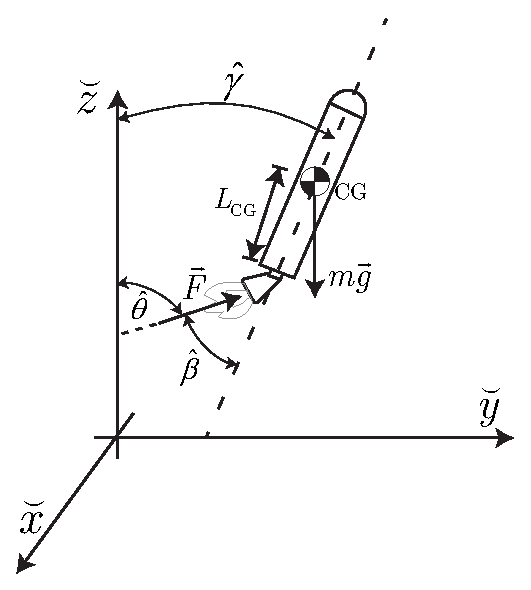
\includegraphics[width=9cm]{fig/rocketFBD.eps}
	\caption{Free Body Diagram for 2D rocket}
	\label{fig:FBD2D}
\end{figure}

\subsection{Modelado matemático}
We start by stating the equations of motion of a 2D rocket with angular control over thrust.

\[
\left\{
\begin{array}{l}
	\ddot{y}=\frac{F}{m} \sin(\gamma+\beta) \\
	\ddot{z}=\frac{F}{m} \cos (\gamma+\beta)-g \\
	\ddot{\gamma} = \frac{L_{\CG}\cdot F}{I_{xx}}\sin\beta
\end{array}
\right.
\]
where \(\LCG\) and \(F\) are a function of time, $m =m_0 - \int \dot{m} $ and $\theta = \gamma+\beta$. 

It is worth clarifying the following will not be taken into account:
\begin{itemize}
	\item Air resistance (drag force)
	\item Wind effects
	\item Fuel sloshing
	\item Relativistic effects
\end{itemize}

We then linearize the equations around a stable operating zone, \textbf{a vertical, still rocket}.\footnote{Modifications to system will need to be made if rocket is to be an orbital delivery device.} This way  small angle relations will be a reasonable approximation.

System linearization around steady point:
\begin{align*}
	\gamma^* = 0 \\
	\beta^* = 0 \\
	F^* = mg
\end{align*}
this way our state space variable for $F$ will be the deviation or peturbation from the steady point. From now on $\Delta F = F- mg$
\subsection{Representación en espacio de estados}
It follows that the number of state-space variables be equal to the number of independent energy storage elements. These are as follows

\begin{enumerate}
	\item[$z$] Gravitation potential energy
	\item[$\dot{y},\dot{z}$] Kinetic energy of rocket
	\item[$\dot{\gamma}$] Angular momentum of rocket
\end{enumerate}
thus, state-space variables are chosen as follows
\begin{align*}
	x_1 = y \\
	x_2 = \dot{y} \\
	x_3 = z \\
	x_4 = \dot{z} \\
	x_5 = \gamma \\
	x_6 = \dot{\gamma}
\end{align*}
where $\dot{x_1} = x_2$, $\dot{x_3} = x_4$ and $\dot{x_5} = x_6$

Let us recall the following Taylor expansion for linearization of trigonometric expressions.
\[
\sin(x+y)|_{x=x_0+\Delta x,y=y_0+\Delta y} \approx \sin(x_0+y_0) + \cos(x_0 + y_0) (x-x_0) + \cos(x_0 + y_0) (y-y_0)
\]
The linearized dynamic equation of the second, third and fourth state are given by the equations of motion mentioned at the start of this document. Below are all the state equations
\begin{equation}
	\dot{x_2} = \frac{F}{m} \left( \gamma+\beta \right) = g x_5 + g u_2 
\end{equation}
\begin{equation}
\dot{x_4} = \frac{F}{m} - g =\frac{F-F_0}{m}= \frac{u_1}{m}
\end{equation}
\begin{equation}
\dot{x_6} = \frac{\LCG \cdot F}{I_{xx}} \beta = \frac{\LCG \cdot mg}{I_{xx}} u_2 
\end{equation}

where $\Ts$ is the sampling time.

The input and output vectors are 
\[
\Cme{u}(t) = \begin{bmatrix}
u_1 \\
u_2
\end{bmatrix} = \begin{bmatrix}
\Delta F \\
\beta
\end{bmatrix}
\]
\[
\Cme{y}(t) = \begin{bmatrix}
y_1 \\
y_2 \\
y_3
\end{bmatrix} = \begin{bmatrix}
y \\
z \\
\gamma
\end{bmatrix}
\]
such that the output equations are

\begin{equation}
	y_1 = x_1 
\end{equation}
\begin{equation}
	y_2 = x_3
\end{equation}
\begin{equation}
	y_3 = x_5
\end{equation}

The matrices are then written ($\Mme{D} = [0]$)
\begin{equation} \label{eq:ssmatrices}
	\Mme{A} = 
	\left[\begin{array}{cccccc} 0 & 1 & 0 & 0 & 0 & 0\\ 0 & 0 & 0 & 0 & g & 0\\ 0 & 0 & 0 & 1 & 0 & 0\\ 0 & 0 & 0 & 0 & 0 & 0\\ 0 & 0 & 0 & 0 & 0 & 1\\ 0 & 0 & 0 & 0 & 0 & 0 \end{array}\right],\quad \Mme{B} = 
	\left[\begin{array}{cc} 0 & 0\\ 0 & g\\ 0 & 0\\ \frac{1}{m} & 0\\ 0 & 0\\ 0 & \frac{\LCG \cdot mg}{I_{xx}} \end{array}\right], \quad \Mme{C} =  \left[\begin{array}{cccccc} 1 & 0 & 0 & 0 & 0 & 0\\ 0 & 0 & 1 & 0 & 0 & 0\\ 0 & 0 & 0 & 0 & 1 & 0 \end{array}\right]
\end{equation}
The system shown in \eqref{eq:ssmatrices} is fully state controllable.
